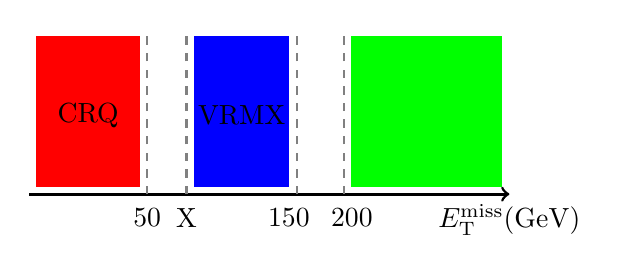
\begin{tikzpicture}[domain=0:4]

  \tikzstyle{region} = [fill]

  \draw[line width=1, ->] (0,0) -- (6.1,0) node[below] {$E_\mathrm{T}^\mathrm{miss} (\mathrm{GeV})$};
  %% \draw[line width=1, ->] (0,0) -- (0,3.1);

  \draw[gray, dashed, line width=0.8] (1.5, 0) -- (1.5, 2.1);
  \draw[gray, dashed, line width=0.8] (4.0, 0) -- (4.0, 2.1);
  \draw[gray, dashed, line width=0.8] (2.0, 0) -- (2.0, 2.1);
  \draw[gray, dashed, line width=0.8] (3.4, 0) -- (3.4, 2.1);

  \node at (1.5,-0.3) {50};
  \node at (2.0,-0.3) {X};
  \node at (3.3,-0.3) {150};
  \node at (4.1,-0.3) {200};

  \draw[green, region] (4.1,0.1) rectangle (6,2);
  \draw node at (5.0,1) {\SRL};

  \draw[red, region] (0.1,0.1) rectangle (1.4,2) ;
  \draw node at (0.75, 1) {CRQ};

  \draw[blue, region] (2.1,0.1) rectangle (3.3,2) ;
  \draw node at (2.7,1) {VRMX};


\end{tikzpicture}
